\documentclass[12pt,a4paper]{article}
\usepackage{amsmath}
\usepackage{amsfonts}
\usepackage{amssymb}
\usepackage{graphicx}
\usepackage{secdot}
\usepackage{amsmath}
\usepackage{commath}
\usepackage[left=2cm,right=2cm,top=2cm,bottom=2cm]{geometry}

\author{ Shibayan Biswas, AE21B109\\ Department of Aerospace Engineering\\ IIT Madras}
\title{Assignment - 6}
\date{October 11, 2022}
\begin{document}
\maketitle
\hline
\section{Introduction:}
In this particular assignment we have been given certain tasks related to be performed on the integral "I" given below and evaluation of errors is possible as the exact value of the integral is known:
\begin{equation}
	\text{I} = \int_{-1}^{1}{ \text{f}(x) \text{dx}}
\end{equation}
The function $f(x)$ is given by the equation shown below:
\begin{equation}
    \text{f}(x) = \text{$e^{-x}$} \text{$\sin^2(4x)$}
\end{equation}
While finding the integral "I" for this particular function $f(x)$, the error is defined by the equation given below:
\begin{equation}
    \text{Error} = \abs{\text{$\int_{-1}^{1}{ \text{f}(x) \text{dx}} - \sum_{i=1}^{N} \text{$f$}(x_i) \text{$w_i$}$}}
\end{equation}
In mathematics, an integral assigns numbers to functions in a way that describes displacement, area, volume, and other concepts that arise by combining infinitesimal data. The process of finding integrals is called integration. Along with differentiation, integration is a fundamental, essential operation of calculus, and serves as a tool to solve problems in mathematics and physics involving the area of an arbitrary shape, the length of a curve, and the volume of a solid, among others.\\
\\The integrals enumerated here are those termed definite integrals, which can be interpreted as the signed area of the region in the plane that is bounded by the graph of a given function between two points in the real line. Conventionally, areas above the horizontal axis of the plane are positive while areas below are negative. Integrals also refer to the concept of an anti-derivative, a function whose derivative is the given function. In this case, they are called indefinite integrals. The fundamental theorem of calculus relates definite integrals with differentiation and provides a method to compute the definite integral of a function when its anti-derivative is known.\\
\\In this particular report I have explicitly written about the tasks to be performed on the integral "I" for this assignment.
\clearpage
\section{Plot of the first five Legendre Polynomials:}
In physical science and mathematics, Legendre polynomials (named after Adrien-Marie Legendre, who discovered them in 1782) are a system of complete and orthogonal polynomials, with a vast number of mathematical properties, and numerous applications. They can be defined in many ways, and the various definitions highlight different aspects as well as suggest generalizations and connections to different mathematical structures and physical and numerical applications.\\
\\Closely related to the Legendre polynomials are associated Legendre polynomials, Legendre functions, Legendre functions of the second kind, and associated Legendre functions.\\
\\In this approach, the polynomials are defined as an orthogonal system with respect to the weight function $w(x) = 1$ over the interval $[-1, 1]$. That is, $P_n(x)$ is a polynomial of degree $n$, such that:
\begin{equation}
    \int_{-1}^{1}{\text{$P_m$}(x) \text{$P_n$}(x) \text{$dx$}} = \text{0}
\end{equation}
In the above equation the point that is to be noted is that $m \neq n$.\\
\\In this section I have provided the plot of the first five Legendre Polynomials which is shown below:
\begin{figure}[!ht]
	\begin{center}
		\framebox{
			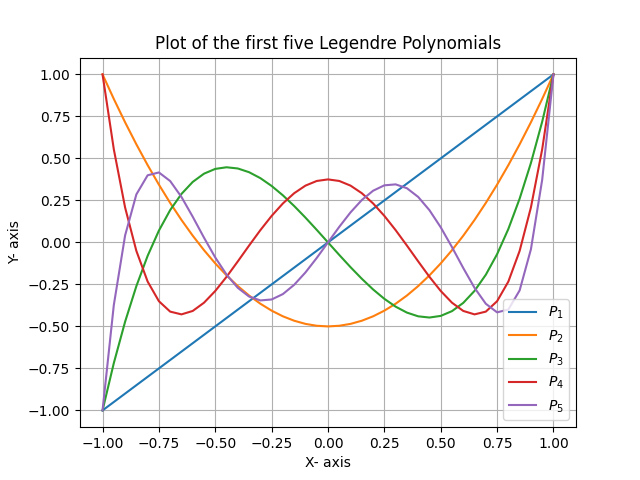
\includegraphics[scale=1.0]{Figure_1.png}
		}
	\end{center}
	\caption{Plot of the first five Legendre Polynomials}
\end{figure}
\clearpage
\section{Plot of  Logarithm of Error v/s number of terms in the series (N):}
In this section I have represented the plot of  Logarithm of Error v/s number of terms in the series (N). In this case I have taken a random value as input for the number of terms in the series (N). For this input value I have got the following plot shown below:
\begin{figure}[!ht]
	\begin{center}
		\framebox{
			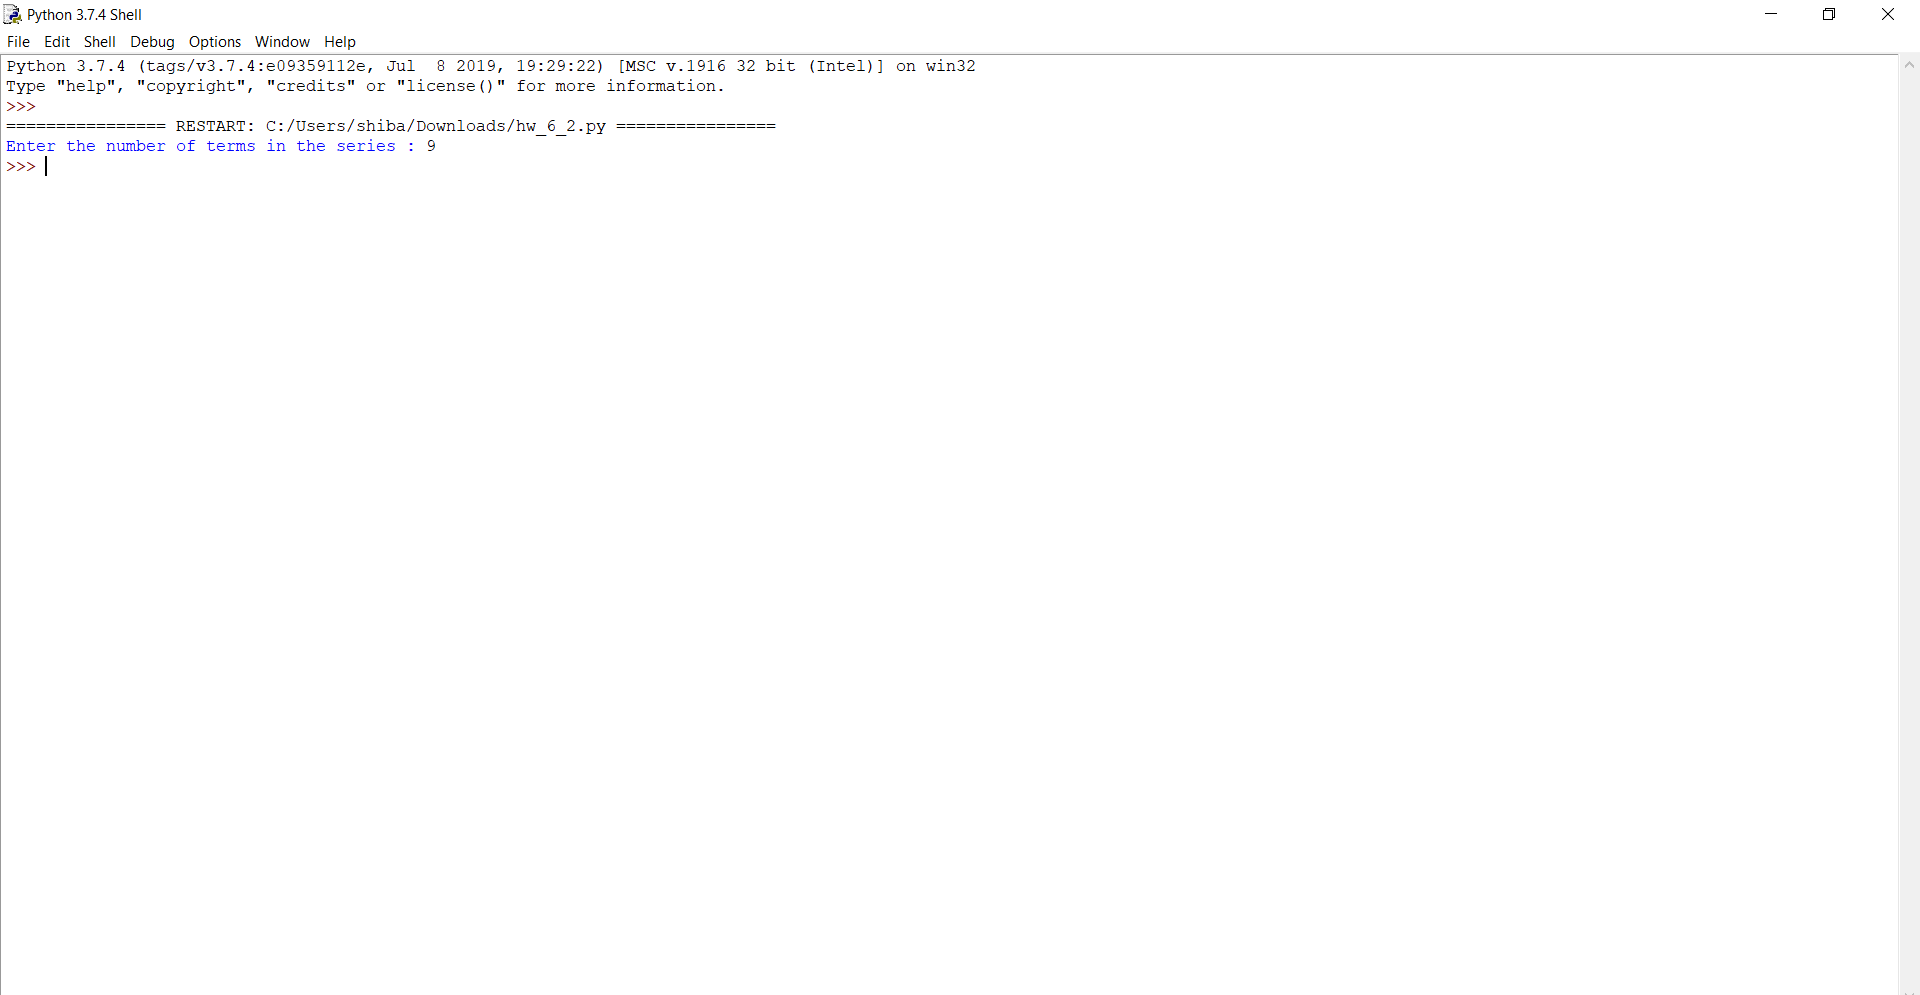
\includegraphics[scale=0.3]{Figure_3.png}
		}
	\end{center}
	\caption{User input data for he number of terms in the series (N)}
\end{figure}
\begin{figure}[!ht]
	\begin{center}
		\framebox{
			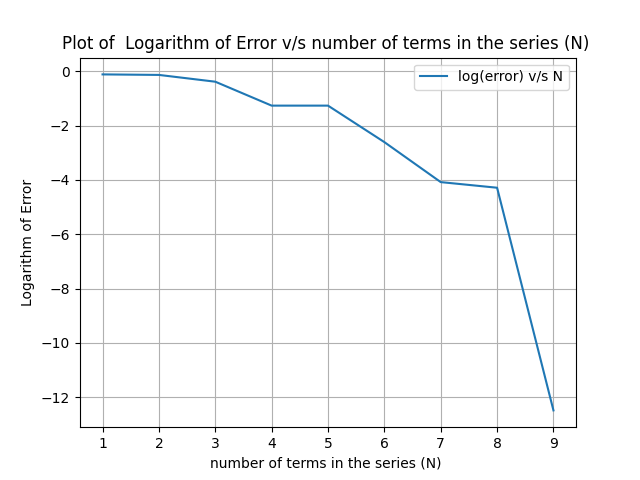
\includegraphics[scale=0.8]{Figure_2.png}
		}
	\end{center}
	\caption{Plot of  Logarithm of Error v/s number of terms in the series (N)}
\end{figure}
\clearpage
\noindent
In the above plot I observe a Monotonic decrease in Error with number of terms in the series. This happens because the property of "scipy.special.roots\textunderscore legendre" is such that when the value of the number of terms in the series (N) is increased then we get more precised values for the Roots and Weights. This leads to a decrease in the Error values and hence the Logarithm of the error values also decreases Monotonically.
\section{Plot of Number of Quadrature Points required (N) v/s Target Error Range :}
In this section I have represented the plot of the Number of Quadrature Points required (N) v/s Target Error Range $\epsilon$ [$10^{-4}, 10^{-1}$] for the Current (Legendre) Method and the Best (Trapezoid) Method. I have considered the Trapezoid Method as the best method, from the previous assignment because the value of Quadrature obtained from the Trapezoid Method has the least possible error compared to the other methods of Quadrature. The plot of the Number of Quadrature Points required (N) v/s Target Error Range $\epsilon$ [$10^{-4}, 10^{-1}$] for the Current (Legendre) Method and the Best (Trapezoid) Method is shown below:
\\ \\
\begin{figure}[!ht]
	\begin{center}
		\framebox{
			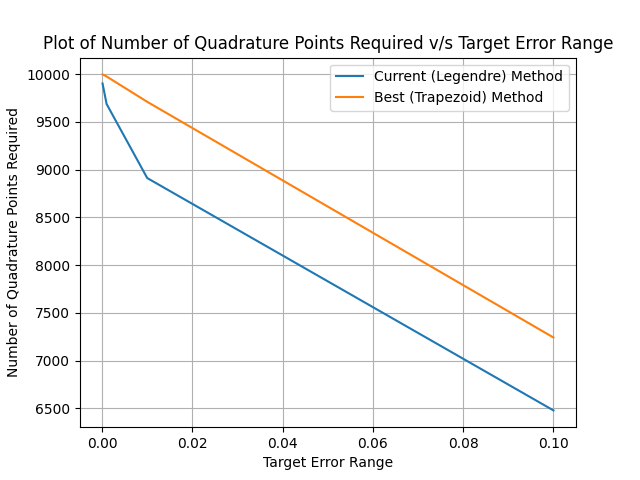
\includegraphics[scale=0.95]{Figure_4.png}
		}
	\end{center}
	\caption{Plot of the Number of Quadrature Points required (N) v/s Target Error Range}
\end{figure}
\clearpage
\section{Plot of  Computational Time required v/s Target Error Range :}
In this section I have represented the plot of the Computational Time required v/s Target Error Range $\epsilon$ [$10^{-4}, 10^{-1}$] for the Current (Legendre) Method and the Best (Trapezoid) Method. I have considered the Trapezoid Method as the best method, from the previous assignment because the value of Quadrature obtained from the Trapezoid Method has the least possible error compared to the other methods of Quadrature. The plot of the Computational Time required v/s Target Error Range $\epsilon$ [$10^{-4}, 10^{-1}$] for the Current (Legendre) Method and the Best (Trapezoid) Method is shown below:
\\ \\
\begin{figure}[!ht]
	\begin{center}
		\framebox{
			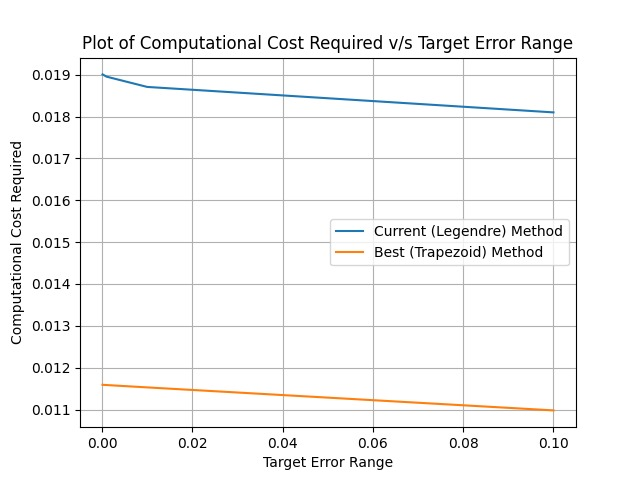
\includegraphics[scale=0.7]{Figure_5.jpg}
		}
	\end{center}
	\caption{Plot of Computational Time required v/s Target Error Range}
\end{figure}
\end{document}
